\documentclass[english, 11pt]{article}
\usepackage{../../notes}
\usepackage{lipsum}

%Global Course Variables
\newcommand{\myCourseCode}{EECS 281}
\newcommand{\myCourseName}{Data Structures and Algorithms}
\newcommand{\myProf}{David Paoletti \& Marcus Darden}
\newcommand{\myTerm}{Winter 2015}
\newcommand{\myLogo}{../um_seal.png}

%Headers
\lhead{\myCourseName}
\rhead{\fancyplain{}{\rightmark}} 

%Footers
\cfoot{\thepage}

\begin{document}
\titleHeader{\myCourseCode}{\myCourseName}{\myProf}{\myTerm}{\myLogo}

%Document information
\noindent\rule{1\columnwidth}{.5pt}
Contributors: Steven Schmatz, Max Smith
\begin{center}
	Latest revision: \today
\end{center}
\toc
\abstr{EECS 281 is an introductory course in data structures and algorithms at the undergraduate level. The objective of the course is to present a number of fundamental techniques to solve common programming problems. For each of these problems, we will determine an abstract specification for a solution and examine one or more potential representations to implement the abstract specification, focusing on those with significant advantages in time/space required to solve large problem instances. When appropriate, we will consider special cases of a general problem that admit particularly elegant solutions.}

%----------------------------
%Document Begins
%----------------------------

\section{Introduction and Workflow}

\section{Complexity Analysis}
	\subsection{Notation}
\begin{itemize}
	\item $x\in\mathbb{R}^D$: data 
	\item $\phi (x)\in\mathbb{R}^M$: features for $\vec{x}$
	\item $t\in\mathbb{R}$: continuous-valued labels
	\item $\vec{x}^{(n)}\equiv \vec{x}_n$: n-th training example
	\item $\vec{t}^{(n)}\equiv \vec{t}_n$: n-th targe value
\end{itemize}

\subsection{1D Inputs}
\begin{itemize}
	\item In the 1D case ($x\in\mathbb{R}^1$)
	\item Given a set of observations $x^{(1)},\ldots ,x^{(N)}$ and corresponding targe values $t^{(1)},\ldots,t^{(N)}$
	\item We want to learn a function $y(\vec{x}, W)\approx t$ to predict future values
	$$y(\vec{x}, \vec{w})=\sum_{j=0}^{M-1}\vec{w}_j \phi_j (\vec{x}) = \vec{w}^T \phi(x)$$
	\item e.g., (green = solution, red = 3-rd polynomial approximation)
	\begin{center}
		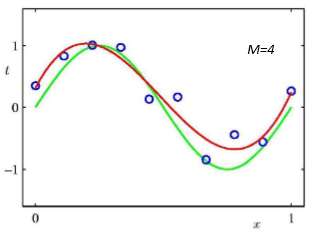
\includegraphics{sections/lec2/3.png}
	\end{center}
	\item For simplicity, we add a \textit{bias function}: $\phi_0 (\vec{x})=1$
	$$\vec{\phi}=1, x, x^2, x^3, \ldots$$
\end{itemize}

\subsection{Basis Function}
\begin{itemize}
	\item Function to construct features from raw data.
	\item e.g.,
	\begin{itemize}
		\item Polynomial: $\phi_j(x)=x^j$
		\item Gaussian: $\phi_j(x)=exp(-\frac{(x-\mu_j)^2}{2s^2})$
		\item Sigmoid: $\phi_j(x)=\sigma (\frac{x-\mu_j}{s})$
	\end{itemize}
\end{itemize}

\subsection{Objective Function}
\begin{itemize}
	\item We will use of sum-of-square errors:
	$$E(w)=\frac{1}{2}\sum_{n=1}^N (y(x^{(n)}, w)-t^{(n)})^2$$
\end{itemize}

\subsection{Batch Gradient Descent}
\begin{itemize}
	\item Given data $(x,y)$ initial $w$, repeat until convergence:
	$$\vec{w}=\vec{w}-\eta \nabla_{\vec{w}} E(\vec{w})$$
	$$\nabla_{\vec{w}}E(w)=\sum_{n=1}^N \left( \sum_{k=0}^{M-1} w_k \phi_k (\vec{x}^{(n)}) - t^{(n)} \right)\phi (\vec{x}^{(n)})=\sum_{n=1}^N \left(\vec{w}^T \phi (\vec{x}^{(n)}) - \vec{t}^{(n)}\right) \phi(x^{(n)})$$
\end{itemize}

\subsection{Overfitting}
\begin{itemize}
	\item An implicit way to tell is when the coeffecients become unreasonably large
	\item Solutions:
	\begin{itemize}
		\item Reduce order
		\item Add more data point
		\item Reselect features, some may be harming you
	\end{itemize}
	\item If you have a small number of data points, then you should use low order polynomial (small number of features)
	\item As you obtain more data points, you can gradually increase the order of the polynomial (more features)
	\item Controlling model complexity: \textbf{regularization}
\end{itemize}

\section{Measuring Runtime, and Pseudocode}
	\subsection{Another kind of factorial}
\begin{lstlisting}[style=C++]
int fact_helper(intn, intresult){
	// REQUIRES: n >= 0
	// EFFECTS: returns result * n!

	if (n == 0) {
		return result;
	}else {
		return fact_helper(n-1,result*n);
	}
}

int factorial(intnum){
	// REQUIRES: num>= 0
	// EFFECTS: returns num!

	return fact_helper(num, 1);
}
\end{lstlisting}

\subsection{Stack effects}
\begin{itemize}
	\item Trace out the stack calls for \lstinline[style=C++]{factorial(2)} for our new and ``old'' function:
	\begin{center}
		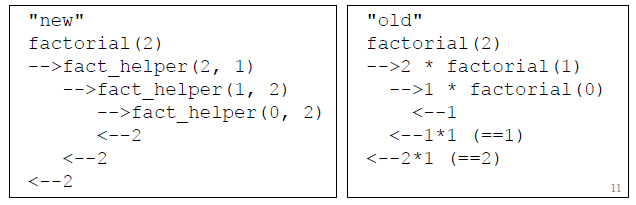
\includegraphics[scale=0.7]{sections/lec3/fact.png}	
	\end{center}

	\item Effects of the new version on the stack:
	\begin{itemize}
		\item The activation record of a function is needed only as long as there is computation left over and can be discarded as soon as the return value is known.
		\item With the new version, the concrete return value isn’t known at the time of the recursive call. However, we do know that whatever that recursive call returns, that will be our return value too.
		\item This means that the caller's stack frame isn't needed any more, and we can throw it away.
	\end{itemize}

	\item This is called \textbf{tail recursion}.
	\item If the result of the recursive call is returned directly with no pending computation, it is tail-recursive. Otherwise, it’s ``plain'' recursion.
\end{itemize}


\section{Recursion and the Master Theorem}
	\subsection{Tail-recursion to iteration conversion}
\begin{itemize}
	\item There are five steps to the conversion of a tail-recursive function to an iterative one:
	\begin{enumerate}
		\item Copy the function's type signature
		\item Identify any needed ``loop variables'' by inspecting the call to the helper function (if it exists).
		\item Write initialization code to mirror the call to the helper function
		\item Identify termination condition(s) and return values by copying the base case behavior.
		\item Write loop body by copying the inductive step
	\end{enumerate}
\end{itemize}

\subsection{Dependency Graphs}
\begin{itemize}
	\item Special kind of graph with ``directed'' edges showing which ``new'' values depend on which ``old'' values.
	\item An edge is drawn from a \textbf{source vertex} to a \textbf{sink vertex}.
	\item To build a dependency graph, draw one vertex for each variable. If variable fooreads from variable barto compute its new value, draw an edge fromfootobar. (Don't draw an edge between a vertex and itself).
	\item If a variable has no edges with it as a sink(i.e. no edges terminate there), you can write its assignment, and erase it and any edges with it as a source.
	\item If two variables (\lstinline[style=C++]{foo, bar}) are each dependent on the other, then you can solve this by inventing shadow variables:
\begin{lstlisting}[style=C++]
int foo_new = bar - 1; // Shadow variable
int bar_new = foo - 1; // Shadow variable
// ------------------
foo = bar_new;
bar = foo_new;
\end{lstlisting}
	\item The transition between these two steps is called a \textbf{software epoch} - dependencies do not exist across epochs.
\end{itemize}

\section{Arrays and Container Classes}
	\subsection{After calibration}
\img{.8}{sections/lec5/p.png}
\begin{itemize}
	\item Internal parameters $K$ are known
	\item $R, T$ are known - but these can only relate $C$ to the calibraiton rig.
	\item You can't estimate $P_i$ from the single image measurement of $p_i$ because it may be anywhere along the line in space.
	\item We also don't have any information in the image to tell us the scale of anything in the world.
\end{itemize}

\subsection{Recovering structure from a single view}
\begin{itemize}
	\item You can make assumptions to get relative sizes of objects in images
	\item Pick a reference plane in the scene
	\item Pick a reference direction (not parallel to the reference plane) in the scene
	\img{.8}{sections/lec5/ref.png}
	\subsubsection{Geometry}
	\img{.8}{sections/lec5/van.png}
	\item Under perspective projection, parallel lines in three-space project to convering lines in the image plane. The common point of intersection, perhaps at infinity, is called the \textbf{vanishing point}
	\begin{itemize}
		\item projection of a point at infinity (goes infinity far)
		\img{.8}{sections/lec5/vp.png}
		\item Any two parallel lines have the same vanishing point
		\item The ray from $C$ through $v$ point is parallel to the lines
		\item AN image may have more than one vanishing point
	\end{itemize}
	\item Two or more vanishing points from lines known to lie in a single 3D plane establish a \textbf{vanishing line}, which completely determines the orientation of the plane
	\img{.7}{sections/lec5/house.png}
\end{itemize}

\subsection{The Cross Ratio}
\img{.8}{sections/lec5/y.png}
\begin{itemize}
	\item $Y$ is desired height to measure
	\item Compute Y from image measurements
	\begin{itemize}
		\item You'll need more than vanishing points to compute this
	\end{itemize}
	\item \textbf{Projective Invariant}: something that does not change under projective transformations (including perspective projection)
	\img{.8}{sections/lec5/l.png}
	\item The \textbf{cross ratio} of 4 collinear points is projective invariant
	$$\frac{||P_3 - P_1||\cdot ||P_4 - P_2||}{||P_3 - P_2||\cdot ||P_4 - P_1||}$$
	\item You can permute the point ordering and it will remain true.
	\item Often called the fundamental invariant of projective geometry
	\img{.8}{sections/lec5/inf.png}
	\item When you consider the points at $\infty$, and the point where the camera would meet the ground plane $v_z$ you have enough points to use the cross ratio on our camera model.
	\item You need the same points in the world and camera system (can't mix and match)
	\item You must make some assumption to determine the relative sizes, typically assume $L$
\end{itemize}

\subsection{Horizon line}
\img{.7}{sections/lec5/hor.png}
\begin{itemize}
	\item Sets of parallel lines on the same plane lead to collinear vanishing points the line is called the \textbf{horizon}
	\img{.8}{sections/lec5/ex.png}
	\item When trying to recover the structure within the camera reference system, we can check if two linesare parallel or not
	\begin{itemize}
		\item If they do, recognize the horizon line
		\item Measure if hte 2 lines meet the horizon
		\item If they do, they are parallel in 3D
		\item Actual scale of scene is not recovered, only relative distances
	\end{itemize}
\end{itemize}

\subsection{Lines in a 2D plane}
$$ax+by+c=0; l=\begin{bmatrix}
	a\\b\\c
\end{bmatrix}$$
\subsubsection{Intersecting lines}
\img{1}{sections/lec5/intersect.png}
\begin{itemize}
	\item The intersection of lines can be calculated with: 
	$$x=l\times l'$$
\end{itemize}

\subsection{Stereo-view geometry}
\img{1}{sections/lec5/tri.png}
\begin{itemize}
	\item Two camera perspectives allow us to find position of objects through \textbf{triangulation}
	\begin{itemize}
		\item This requires a few knowns, $K_1, K_2, R, T$
	\end{itemize}
	\item Small inaccuracies with knowns can lead to situations where the lines may not intersect 
	\item Instead, we'll find where they came close enough
		$$d^2(x_1, M_1X)+d^2(x_2, M_2X)$$
		$$d:=\text{distance between two lines}$$
\end{itemize}

\subsection{Epipolar Geometry}
\img{.7}{sections/lec5/ep.png}
\begin{itemize}
	\item \textbf{Epipolar plane} (grey): intersections of baseline with image planes
	\item \textbf{Baseline} (orange): projectison of other camera center
	\item \textbf{Epipolar lines} (blue): vanishing points of camera motion direction
	\item This framepoint, allows us to consider if two pointsare related by epipolar geometry
	\item Use epipolar lines to find sharing points will greatly save computation cost as a 2D search becomes 1D
	\subsubsection{Parallel image planes}
	\item Baseline intersects the image plane at infinity
	\item Epipoles are at infinity
	\item Epipolar lines are parallel to x-axis
	\subsubsection{Forward translation}
	\img{1}{sections/lec5/f.png}
	\item When a camera moves forward the lines turn into a spiral
\end{itemize}

\section{Linked Lists and Iterators}
	\subsection{Recap - Bounds Checking for Arrays Example}
\subsubsection{Basic Layout}
\begin{lstlisting}[style=C++]
class Array {
 public:
    Array(unsigned len = 0) : length(len) {
        data = (len ? new double[len] : nullptr);
    }
 private:
    double *data;        // array data
    unsigned int length; // array size
}
\end{lstlisting}
You could use a struct, but users of your class would be able to access all member variables of your struct by default.

\subsubsection{Copy Constructor}
To copy the array, you need to perform a \textit{deep copy}:
\begin{lstlisting}[style=C++]
Array(const Array & a) {
    length = a.getLength(); // getter for length // 1 step
    data = new double[length];                   // 1 step
    for (unsigned i = 0; i < length; i++) {      // n times
        data[i] = a[i];                          // c steps
    }
}
\end{lstlisting}
The complexity of this is: $\O{! + 1 + (nc) + 1}=\O{n}$

\subsubsection{Better Copying}
\begin{lstlisting}[style=C++]
void copyFrom(const Array & a) {
    if (length != a.length) {
        delete[] data;
        length = a.length;
        data = new double[length];
    }

    for (unsigned int i = 0; i < length; i++) {
        data[i] = a.data[i];
    }
}

Array(const Array & a) : length(0), data(nullptr) {
    copyFrom(a);
}

Array & operator=(const Array & a) {
    copyFrom(a);
    return *this;
}
\end{lstlisting}

\subsection{The Big 5}
\begin{itemize}
	\item Destructor
	\item Copy constructor
	\item Overloaded operator=
	\item Copy constructor from \textit{r-value}
	\item Overloaded operator= from \textit{r-value}
\end{itemize}

\subsubsection{Destructor}
\begin{lstlisting}[style=C++]
~Array() {
    if (data != nullptr) {
        for (int i = 0; i < length; i++) { // n times
            delete data[i];                // 1 step
        }
        delete[] date;                     // 1 step
        data = nullptr;                    // 1 step
    }
}
\end{lstlisting}
Complexity: $\O{n}$

\subsubsection{Access Operator[]}
\begin{lstlisting}[style=C++]
const double & operator[](int idx) const {
    if (idx < length && idx >= 0)
        return data[idx];
    throw runtime_error("bad idx");
}
\end{lstlisting}
\begin{itemize}
	\item Declares read-only access/
	\item Automatically selected by the compiler when an array being access is marked \lstinline[style=C++]{const}
	\item Helps compiler optimize code for speed
	\item Some functions, like \lstinline[style=C++]{ostream &operator<<(ostream &os, const Array &a)} require \lstinline[style=C++]{const}.
	\item Must also make a non-constr version
\end{itemize}

\subsubsection{Access with more than 2 dimensions}
\begin{lstlisting}[style=C++]
const double &operator()(int i, int j) const {
    // return by const reference
}
\end{lstlisting}
\begin{itemize}
	\item Can't overload \lstinline[style=C++]{operator[][]}
\end{itemize}

\subsubsection{Inserting an Element}
\begin{lstlisting}[style=C++]
bool insert(int index, double val) {
    if (index >= size || index < 0) {
        return false;
    } else {
        for (int i = size - 1; i > index; --i) {
            data[i] = data[i - 1];
        }
        data[index] = val;
        return true;
    }
}
\end{lstlisting}
Complexity:
\begin{itemize}
	\item Best case: $\O{1}$
	\begin{itemize}
		\item The element is inserted at the end
	\end{itemize}

	\item Average case: $\O{n}$
	\begin{itemize}
		\item Go through half of elements (but that is a constant times $n$)
	\end{itemize}

	\item Worst case: $\O{n}$
	\begin{itemize}
		\item Go through all elements
	\end{itemize}
\end{itemize}

\subsubsection{Append}
When array is full, resize:
\begin{itemize}
	\item Double array size from $n$ to $2n$
	\item Copy $n$ items from the original array to the new array
	\item Appending $n$ elements
	\item Total: $1 + n + n = 2n + 1$ steps
	\item Amortized: $(2n+1)/n=\O{1}$ steps
\end{itemize}

\subsection{Linked Lists and Iterators}
\begin{itemize}
	\item \textbf{Linked list}: Each person points to the next person
	\item \textbf{Doubly linked list}: Each person points to each other
	\item \textbf{Circularly linked list}: A list which has the first and last nodes pointing to each other
\end{itemize}

\subsubsection{Arrays vs Linked Lists}
Arrays:
\begin{itemize}
	\item Access:
	\begin{itemize}
		\item Random: $\O{1}$ time
		\item Sequential: $\O{1}$ time
	\end{itemize}

	\item Insert:
	\begin{itemize}
		\item Insert: $\O{n}$ time
		\item Append: $\O{n}$ time
	\end{itemize}

	\item Book-keeping:
	\begin{itemize}
		\item \lstinline[style=C++]{ptr} to beginning
		\item \lstinline[style=C++]{current_size} or \lstinline[style=C++]{ptr}
		\item \lstinline[style=C++]{max_size} or \lstinline[style=C++]{ptr} to end off allocated space
	\end{itemize}

	\item Memory:
	\begin{itemize}
		\item Wastes memory if size is too large
		\item Requires reallocation if too small
	\end{itemize}
\end{itemize}
Linked Lists:
\begin{itemize}
	\item Access:
	\begin{itemize}
		\item Random: $\O{n}$ time
		\item Sequential: $\O{1}$ time
	\end{itemize}

	\item Insert:
	\begin{itemize}
		\item Insert: $\O{n}$ time
		\item Append: $\O{1}$ time
		\begin{itemize}
			\item Append to \lstinline[style=C++]{tail_ptr}
		\end{itemize}
	\end{itemize}

	\item Book-keeping:
	\begin{itemize}
		\item \lstinline[style=C++]{head_ptr} to first node
		\item \lstinline[style=C++]{size} (optional)
		\item \lstinline[style=C++]{tail_ptr} to last node
		\item In each node, \lstinline[style=C++]{ptr} to next node
		\item Wasteful for small data times (overhead on pointers)
	\end{itemize}

	\item Memory:
	\begin{itemize}
		\item Allocates memory as needed
		\item Requires memory for pointers
	\end{itemize}
\end{itemize}

\subsection{Linked List Implementation}
\begin{lstlisting}[style=C++]
class LinkedList {
 public:
    LinkedList();
    ~LinkedList();
 private:
    struct Node {
        double item;
        Node *next;
        Node() {next = nullptr;}
    };

    Node *head_ptr;
};
\end{lstlisting}

\subsubsection{Methods}
\begin{lstlisting}[style=C++]
int size() const;

bool append_item(double item);
bool append_node(Node *n);

bool delete_item(double item);
bool delete_node(Node *n);
\end{lstlisting}

\subsubsection{Maintaining Consistency}
Arrays:
\begin{itemize}
	\item Stored size matches number of elements at all times
	\item Be sure that \lstinline[style=C++]{start_ptr + size < end_ptr}
\end{itemize}
Linked Lists
\begin{itemize}
	\item Stored size matches number of elements
	\item The last node points to \lstinline[style=C++]{nullptr}
	\item If the list is a circular list, last node points to head
	\item If a doubly-linked list, next/prev pointers are consistent
\end{itemize}

\section{The Standard Template Library}
	\subsection{Passing Pointers to Functions}
\begin{itemize}
	\item Pointers can be arguments to functions. For example, suppose you want a function that adds one to an integer argument passed by reference:
\begin{lstlisting}[style=C++]
void add_one(int *x){
	// MODIFIES: *x
	// EFFECTS: adds one to *x
	*x = *x + 1;
}
\end{lstlisting}
	\item If you were to call this function as so: \lstinline[style=C++]{add_one(bar);}, where \lstinline[style=C++]{bar} is a pointer to \lstinline[style=C++]{foo}
\begin{lstlisting}[style=C++]
int foo;
int *bar;
bar = &foo;

add_one(bar);
\end{lstlisting}
	\begin{itemize}
		\item The variable bar is bassed by \textbf{value}, but it's a pointer!
		\item Both bar and the copy of bar refer to the same address in memory.
	\end{itemize}
	\item You can also make the call without the ``middleman'' like: \lstinline[style=C++]{add_one(&foo);}
\end{itemize}

\subsection{Pointer question}
\begin{itemize}
	\item If you modify \lstinline[style=C++]{add_one} to:
\begin{lstlisting}[style=C++]
void add_one(int *x){
	x = x + 1;
}
\end{lstlisting}	
	\item It will increment the value \textbf{of the pointer} by one.
	\item Pointer arithmetic is done based on units of the \textbf{referent type} (the type of the objects in the list).
\end{itemize}

\subsection{Pointers vs. references}
\begin{itemize}
	\item Both allow you to pass objects by reference.
	\item Pointers require some extra syntax at calling time (\&), in the argument list (*), and with each use (*); references only require extra syntax in the argument list (\&).
	\item You can change the object to which a pointer points using arithmetic/assignment, but you cannot change the object to which a reference refers.
	\item You might wonder why you’d ever want to use pointers, since theyrequire extra typing, and allow you to shoot yourself in the foot.
	\item Why use pointers?
	\begin{itemize}
		\item Array variables are internally implemented using pointers
		\item They allow us to create structures (unlike arrays) whose size is not known in advance; we won't see that use until the last third of the course.
	\end{itemize}
\end{itemize}

\subsection{Pointers and Arrays}
\begin{itemize}
	\item Arrays are actually represented via pointers as so:
	\begin{center}
		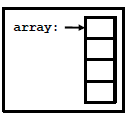
\includegraphics{sections/lec7/array.png}
	\end{center}
	\item If you were to look at the value of the variable ``array'' (not \lstinline[style=C++]{array[0]}) you'd find that it was exactly the same as the address of \lstinline[style=C++]{array[0]}.
	\item When the argument \lstinline[style=C++]{array} is passed to the function sum, a pointer to the first element of the array is really passed and the compiler does all the work of translating something like: \lstinline[style=C++]{array[3]} into the proper arithmetic/dereference to get the right value.
\begin{lstlisting}[style=C++]
x = array[3];
// Is equivalent to:
int *tmp;
tmp = array + 3;
x = *tmp;
// Or simply:
x = *(array + 3);
\end{lstlisting}
\end{itemize}

\subsection{Indexing vs. pointer arithmetic}
\begin{itemize}
	\item Using array indexing:
\begin{lstlisting}[style=C++]
for (int i = 0; i < SIZE; ++i){
	cout << array[i] << " ";
}
\end{lstlisting}
	\item Using pointer arithmetic:
\begin{lstlisting}[style=C++]
for (int *i = array; i < array+SIZE; ++i){
	cout << *i << " ";
}
\end{lstlisting}
\end{itemize}

\subsection{Array Traversal Using Pointers}
\begin{lstlisting}[style=C++]
int strlen(char *s) {
	char *p = s;
	while (*p) ++p;
	return p - s;
}
\end{lstlisting}
\begin{itemize}
	\item \lstinline[style=C++]{*p} evalues to ``false'' if \lstinline[style=C++]{p} points to a NULL, true otherwise.
	\item \lstinline[style=C++]{++p} advances by ``one character''
	\item \lstinline[style=C++]{p-s} computes the ``number of characters'' between \lstinline[style=C++]{p} and \lstinline[style=C++]{s}
\end{itemize}

\subsection{Constants}
\begin{itemize}
	\item \lstinline[style=C++]{void strcpy(char *dest, const char *src);}
	\item \lstinline[style=C++]{const} is a \textbf{type qualifier} - something that modifies a type
	\item It means ``you cannot change this value once you have initialized it.''
	\item When you have pointers, there are two things you might change:
	\begin{itemize}
		\item The value of the pointer.
		\item The value of the object to which the pointer points.
	\end{itemize}
	\item Either (or both) can be made unchangeable:
\begin{lstlisting}[style=C++]
const T *p;			// "T" (the pointed-to object) cannot be changed
T *const p;			// "p" (the pointer) cannot be changed
const T *const p;	// neither can be changed.
\end{lstlisting}
	\item Adding \lstinline[style=C++]{const} will stop changing value mistakes, and the compiler will catch them.
	\item You can use a pointer-to-T anywhere you expect a pointer-to-const-T, but NOT vice versa
	\item That's because code that expects a pointer-to-T might try to change the T, but this is illegal for a pointer-to-const-T.
	\item However, code that expects a pointer-to-const-T will work perfectly well for a pointer-to-T; it's just guaranteed not to try to change it.
\end{itemize}

\subsection{C strings vs. C++ strings}
\begin{center}
\begin{tabular}[breaklines=true]{p{5cm}|p{5cm}|p{5cm}}
	& C string & C++ string \\
	\hline
	Library headers & 
{\begin{lstlisting}[style=C++] 
#include <string>
\end{lstlisting}} & 
{\begin{lstlisting}[style=C++]
#include string
\end{lstlisting}}\\	
	string constant &
{\begin{lstlisting}[style=C++]
constchar* hello = "hello";
\end{lstlisting}}&
{\begin{lstlisting}[style=C++]
conststring hello = "hello";
\end{lstlisting}} \\
	length &
{\begin{lstlisting}[style=C++]
strlen(hello);//5
\end{lstlisting}} &
{\begin{lstlisting}[style=C++]
hello.length();//5
\end{lstlisting}} \\
	local variable &
{\begin{lstlisting}[style=C++]
constintMAXSIZE=1024; 
char s[MAXSIZE];
\end{lstlisting}} &
{\begin{lstlisting}[style=C++]
string s;
\end{lstlisting}} \\
	copy &
{\begin{lstlisting}[style=C++]
strcpy(s, hello);
\end{lstlisting}} &
{\begin{lstlisting}[style=C++]
s = hello;
\end{lstlisting}} \\
	concatenate &
{\begin{lstlisting}[style=C++]
constchar* world = " world";
char message[MAXSIZE];
strcpy(message, hello);
strcat(message, world);
\end{lstlisting}} &
{\begin{lstlisting}[style=C++]
string message = hello + " world";
\end{lstlisting}} \\
	compare &
{\begin{lstlisting}[style=C++]
if (strcmp(a,b) == 0)
	// do something
\end{lstlisting}} &
{\begin{lstlisting}[style=C++]
if (a == b)
	// do something
\end{lstlisting}} \\
	convert to C++ string &
{\begin{lstlisting}[style=C++]
string cpp_str = hello;
\end{lstlisting}} &
{\begin{lstlisting}[style=C++]
char c_str[MAXSIZE];
strcpy(c_str, message.c_str());
\end{lstlisting}} \\
\end{tabular}
\end{center}

\subsection{Type Sizes}
\begin{itemize}
	\item The amount of memory assigned to a data type is a source of innumerable ``portability bugs'' in programs.
	\item There are \textbf{some} guarantees, however:
	\begin{itemize}
		\item A ``char'' is always one byte
		\item A ``short'' is always at least as big as a char
		\item An ``int'' is always at least as big as a short
		\item A ``long'' is always at least as big as an int
	\end{itemize}
	\item \lstinline[style=C++]{sizeof(int)} tells you the number of bytes required to store an \lstinline[style=C++]{int}
	\begin{center}
		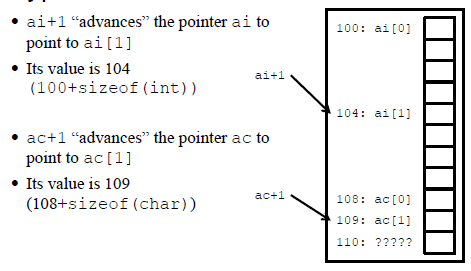
\includegraphics{sections/lec7/type.png}
	\end{center}
\end{itemize}

\end{document}